\documentclass[12pt]{article}

% Packages
\usepackage{sbc-template}
\usepackage{graphicx,url}
\usepackage[brazil]{babel}   
\usepackage[utf8]{inputenc}  
\usepackage{lipsum}

\sloppy

% Info
\title{Albi:\\ A gro compiler to the SBML standard}
\author{Alek Frohlich\inst{1}, Gustavo Biage\inst{1}}
\address{Departamento de Informatica e Estatística – Universidade Federal de Santa Catarina \\
Florianopolis – SC – Brazil
  \email{\{alek.frohlich,gustavo.c.biage\}@grad.ufsc.br}
}

\begin{document}
\maketitle

% Topics:
%       => The growth of the area leads to the development of multicellular devices
%       => Gro is well suited for this purpose
%       => However it isn't ready for compatibility
%       => Introduce the objective of making it compatible
\begin{abstract}


    The growth of research areas such as synthetic biology and systems biology leads to an increased willing to develop new, larger mathematical models to describe complex biological behavior. In order to enable natural flow of development of those models, scientists must have access to tools which increase the level of abstraction and enable reuse of biological components. Increased efforts are being put on solving these two problems. The present work tackles those problems by interfacing the existing programming language gro with SBML for model interchangeability and ease of model representation.


\end{abstract}

% Topics:
%       => What does albi fix that libSBML does not?
%       => What are the reasons we chose gro as albi's primary language?
%       => What are the disadvantages of the gro simulator
%       => What are the advantages of having the SBML model for a gro program?
%       => Prepare next sections
\section{Introduction}


    Even though a Systems Biology Markup Language API library (LibSBML) has already been developed 
    \cite{Bornstein2008}, it only ought to be useful in cases where a new model is to be developed. In cases where 
    there is a preexisting model, on the other hand, the availability of a SBML library doesn't help much since the 
    previous model would have to be entirely rewritten to fit the API. Instead, the present work proposes a language 
    parser that generates SBML code from previously built gro models. gro is a language for programming, modeling, 
    specifying and simulating the behavior of cells in growing micro colonies of microorganisms \cite{Jang2012}. It 
    has been made the primary source of the parser considering it has many interesting syntactical constructs such as
    rate statements, program definitions and bacterial instantiation which can be neatly represented in SBML  
    documents as reactions, local name spaces and compartments, respectively.
    
    % too much its, lacks cohesion at the end
    As language support goes, gro is still tightly coupled with it's original simulator. Although the simulator has 
    recently undergone big improvements making simulations behave more realistically \cite{Gutirrez2017}, it doesn't 
    change the fact that the original simulator is the only available way to validate gro models. This hinders the 
    reproducibility of experiments built with the language. SBML models are now supported by more than 100 simulators \cite{Hucka2007},
    
    Another great opportunity the language was missing is BioModels integration \cite{LeNovere2006}. BioModels is a 
    database of curated SBML and CellML models maintained with the intent of providing researches with models related
    to a particular disease, biological process or molecular complex. If gro code is to be translated into SBML, then
    models written in it are automatically more likely to be peer reviewed or stored as reference models for their 
    respective biological behavior.

    % fix cohesion and formatting
    In the second section, we introduce the parser and show some examples of gro source code being translated to SBML
    models; In the third section, we explain how we used tellurium to generate the SBML; The fourth section, we 
    compile the repressilator into equivalent SBML code and then simulate it in Copasi; Lastly, we conclude by 
    confirming what we've done and proposing future works.
    
    
% Topics:
%       => Which syntax does the parser recognize?
%       => Examples of generated SBML
\section{The parser}
    The parser recognizes a subset of the gro syntax. It does so because the main multicellular features of gro aren't yet supported by SBML, a known single-cell modelling language. That i

\section{The Tellurium framework}
    \lipsum[1]

\section{Study case: The Repressilator}
    \lipsum[1]

\subsection{Mathematical Model}
    \lipsum[1]
    % Cite example
    \cite{Hucka2003}
    % Figure example
    (Figure~\ref{fig:repressilator}).

% Oscillation
\begin{figure}[ht]
\centering
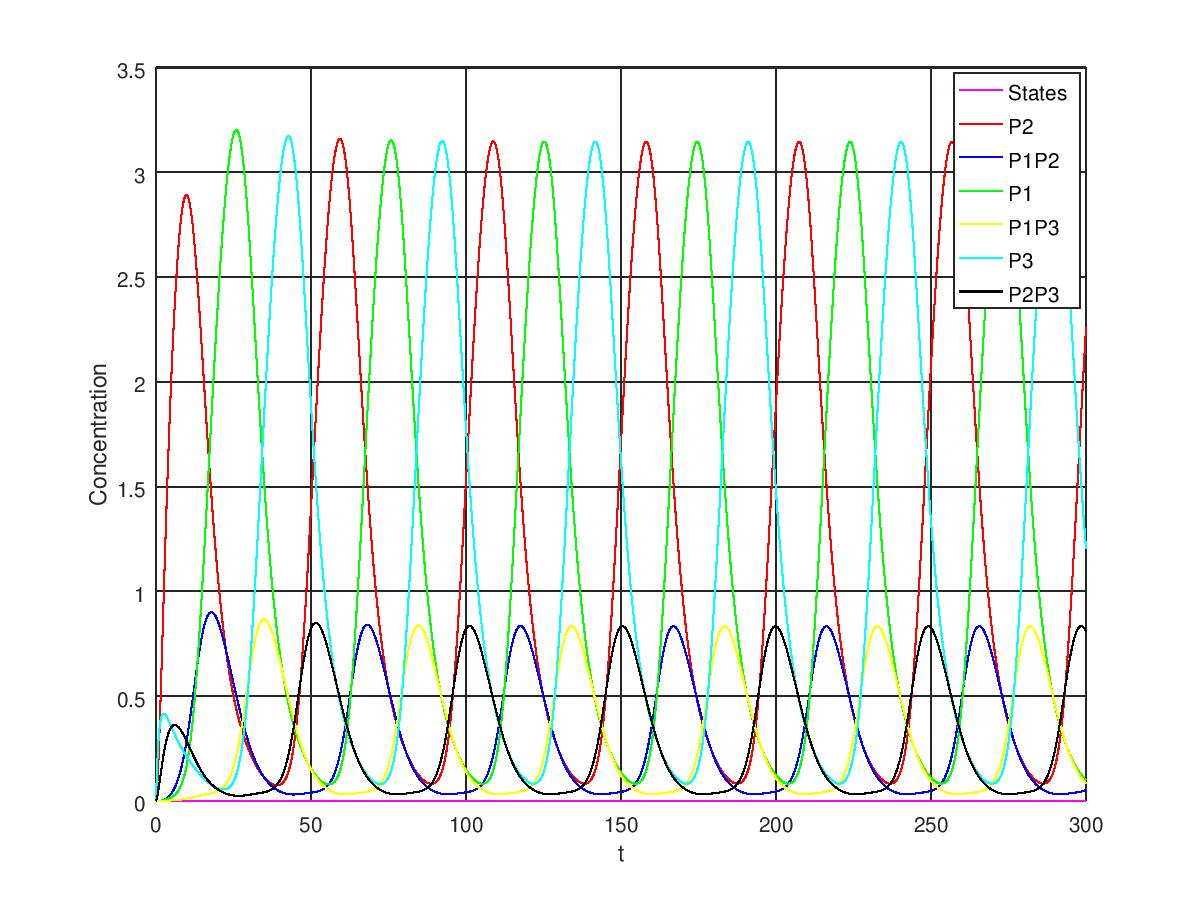
\includegraphics[width=.5\textwidth]{repressilator.jpg}
\caption{Repressilator}
\label{fig:repressilator}
\end{figure}

EPS generated from Octave
\begin{center}
    \begin{figure}[h]
        
        \begin{subfigure}
            \includegraphics[scale = 0.4]{my_plot-inc.eps}
            \caption{Caption1}
            \label{fig:subim1}
        \end{subfigure}
        \begin{subfigure}
            \includegraphics[scale = 0.4]{my_plot-inc.eps}
            \caption{Caption1}
            \label{fig:subim1}
        \end{subfigure}
    \end{figure}
    % \setlength{\unitlength}{1pt}
    % \begin{picture}(0,0)
    % \includegraphics[scale = 0.4]{my_plot-inc}
    % \end{picture}%
    % \begin{picture}(576,432)(0,0)
    % \fontsize{10}{0}
    % \end{picture}
\end{center}

\subsection{Extracting behavior from Gro}
    \lipsum[1]
    
\subsection{Simulating output on Copasi}
    \lipsum[1]

\section{Conclusion}
    \lipsum[1]
    
% Topics:
%       => It would be nice if SBML were to be upgraded to fit multicellular models
%       => Then we could extend the parser's syntax to make gro the multicellular systems biology %              programming language
\section{Future works}
    As it is now, there isn't a multicellular systems biology programming language. The authors believe nonetheless, that gro could be that language, if only a model exchange format such as SBML were to handle it. After that's done, extending the parser's syntax even without the help of APIs in the likes of libSBML and Tellurium, would be a relatively simple task.

% References
\bibliographystyle{sbc}
\bibliography{sbc-template}

\end{document}
